% Origen: Secciones/PI - Implementacion TOP (Integracion).md
\chapter{Implementación del TOP (integración)}
\label{C:top}

% Figuras de ESTE capítulo + las compartidas. Siempre al principio del archivo.
\graphicspath{{figs/cap12/}{figs/comunes/}}

\begin{destacado}
Este capítulo habla de (1) qué es y qué incluye un módulo de integración, (2) el
módulo base original de Pitaya, versión 0.94, en el que nos basamos, y los
cambios aplicados, (3) los posibles caminos que puede tener el datapath y (4)
los registros de configuración del mismo~\cite{RedPitayaFPGA}.
\end{destacado}

%==============================================================================
\section{Sistema base de Pitaya: módulo de integración}
\label{S:top-sistema-base}

Este es el archivo cabecera (TOP) del diseño, y es el responsable de:
\begin{itemize}
  \item Tener como entradas y salidas las interfaces de los periféricos
    externos.
  \item Instanciar macros de recursos de clock y macros de periféricos
    empleados, por ejemplo el PS.
  \item Armar las \textbf{redes de reloj} (\emph{clock domains}) y las
    \textbf{redes de reset} (\emph{reset domains}).
  \item \textbf{Instanciar los módulos e interconectarlos}.
  \item \textbf{Instanciar el bus interno} e interconectarlo mediante un bridge
    al PS.
\end{itemize}

\subsection{Vista general del TOP}
\label{S:top-vista-general}

La documentación oficial~\cite{RedPitayaDocs} presenta el esquema ASCII del
TOP, mientras que el nuestro, \codigo{event\_ring\_red\_pitaya\_top}, se presenta en la
Fig.~\ref{f:top-panorama} y está constituido por los siguientes subsistemas:
\begin{itemize}
  \item \textbf{Módulo del PS}: \codigo{red\_pitaya\_ps}, que pertenecía al
    sistema original de Pitaya.
  \begin{itemize}
    \item Toma las señales físicas del módulo e instancia estructuras que las
      representan.
  \end{itemize}
  \item \textbf{Bridges PS-PL}: el PS y la PL se comunican por dos
    caminos~\cite{UG585}.
  \begin{itemize}
    \item \textbf{Control}, por el puerto maestro M\_AXI\_GP0 del PS. Del lado de
      la PL lo recibe \codigo{axi4\_slave}, que traduce las transacciones
      AXI4-Lite de 32 bits~\cite{AMBAAXI} al handshake del bus custom. Es el
      camino lento, el que usa el ARM para leer y escribir registros.
    \item \textbf{Datos}, por los puertos esclavos S\_AXI\_HP del PS. Del lado
      de la PL los maneja \codigo{axi\_master}, que convierte las escrituras del
      bus custom en ráfagas AXI4 de 64 bits hacia la DDR, sin pasar por el ARM.
      Se usa sólo HP2, por el que el \codigo{event\_ring} escribe sus ventanas.
      HP0 y HP1, los de la captura del OSC a DDR, y HP3 quedan en cero.
  \end{itemize}
  \item \textbf{Interconnect del bus custom}: los detalles de la interfaz y las
    secuencias que utiliza el bus custom se presentan en la
    Sec.~\ref{S:intro-hw-bus-custom}. El interconnect,
    \codigo{sys\_bus\_interconnect}, reparte cada transacción del PS al módulo
    que corresponde.
  \begin{itemize}
    \item Está instanciado de forma que subdivide el espacio de direcciones en 8
      regiones de igual tamaño, de 1~MiB cada una a partir de
      \codigo{0x4000\_0000}. Estas se presentan en la
      Tabla~\ref{t:top-slots}.
  \end{itemize}
\end{itemize}

\begin{figure}[H]
\centering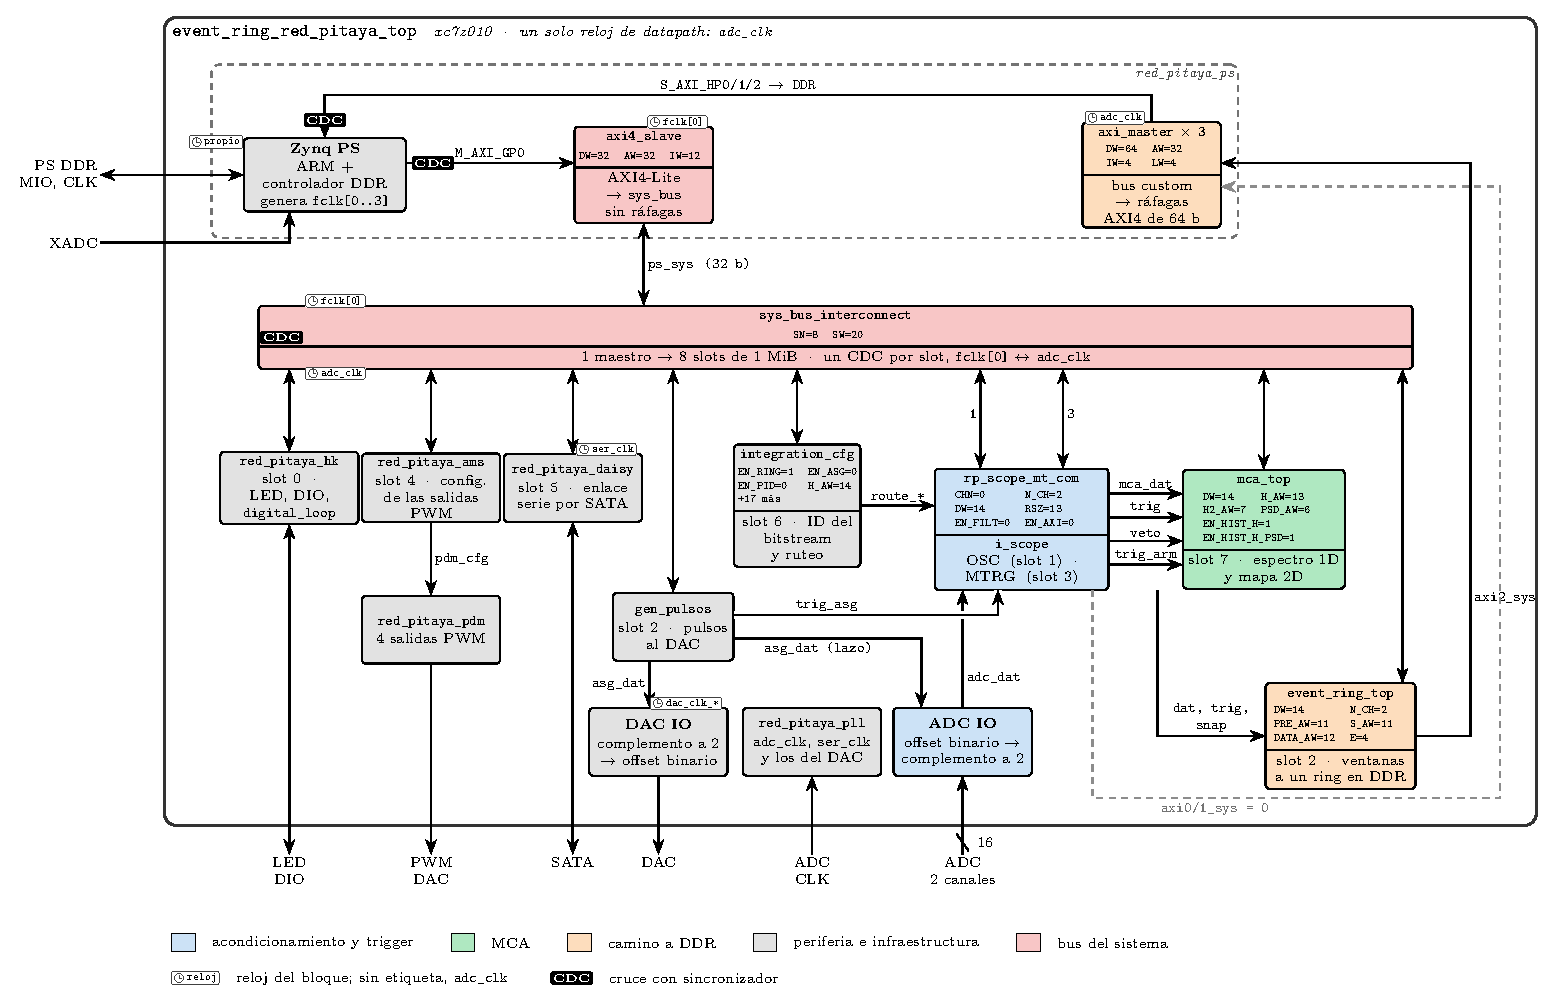
\includegraphics{cap12_panorama_top}
\caption[Diagrama general del TOP del sistema]{%
Diagrama general del TOP del sistema. Los pines físicos quedan en el borde.
Control: GP0 $\rightarrow$ \codigo{sys\_bus}. Datos: \codigo{event\_ring\_top}
$\rightarrow$ HP2 $\rightarrow$ DDR, sin pasar por el ARM; la captura del OSC a
DDR no está (\codigo{EN\_AXI=0}) y \codigo{axi0/1\_sys} quedan en cero.
\codigo{NOMBRE=valor}: parámetros con que el padre instancia el bloque (se
omiten los que sólo pasan el del padre sin cambio). En \codigo{integration\_cfg}
se muestran 4 de sus 21. Las etiquetas con reloj marcan los bloques que no
corren en \codigo{adc\_clk}, o que podrían confundirse: \codigo{axi\_master}
está dentro del PS pero corre en \codigo{adc\_clk}. \codigo{CDC} marca los
cruces que necesitan sincronizador: el interconnect, uno por slot, entre
\codigo{fclk[0]} y \codigo{adc\_clk}, que tienen la misma frecuencia nominal
pero salen de osciladores distintos, y los puertos GP0 y HP, que cruza el propio
PS. El slot 2 lo comparten el \codigo{event\_ring} (\codigo{0x4020\_0000}) y
\codigo{gen\_pulsos} (\codigo{0x4021\_0000}), que maneja el DAC, la fuente ASG
del multitrigger y, con \codigo{digital\_loop[0]}, la entrada de la cadena en
lugar del ADC.\label{f:top-panorama}}
\end{figure}

\begin{table}[H]
\centering
\caption[Regiones del bus custom]{%
Regiones del bus custom en \codigo{event\_ring\_red\_pitaya\_top}. Los slots 1
y 3 son dos buses de la misma instancia, \codigo{rp\_scope\_mt\_com}, que expone
por separado los registros del osciloscopio y los del multitrigger. El slot 2
lo reparte \codigo{sys\_bus\_split}: los 64~kB de \codigo{0x4021\_0000} van a
\codigo{gen\_pulsos} y el resto al \codigo{event\_ring}.\label{t:top-slots}}
\small
\begin{tabularx}{\textwidth}{|c|l|>{\raggedright\arraybackslash}X%
  |>{\raggedright\arraybackslash}p{0.22\textwidth}|}
\hline \encabezado \textbf{Slot} & \textbf{Base} & \textbf{Módulo} &
  \textbf{Origen} \\ \hline
0 & \codigo{0x4000\_0000} & \codigo{red\_pitaya\_hk}: LEDs, DIO y lazo digital
  & Red Pitaya \\ \hline
1 & \codigo{0x4010\_0000} & osciloscopio (\codigo{rp\_scope\_mt\_com}) & Red
  Pitaya, modificado \\ \hline
2 & \codigo{0x4020\_0000} & \codigo{event\_ring} en \codigo{0x4020\_0000};
  \codigo{gen\_pulsos} en \codigo{0x4021\_0000} & propio, en lugar del ASG
  \\ \hline
3 & \codigo{0x4030\_0000} & multitrigger (\codigo{rp\_scope\_mt\_com}) &
  propio, en lugar del PID \\ \hline
4 & \codigo{0x4040\_0000} & \codigo{red\_pitaya\_ams}: XADC y PDM & Red Pitaya
  \\ \hline
5 & \codigo{0x4050\_0000} & \codigo{red\_pitaya\_daisy}: enlace serie por los
  conectores SATA & Red Pitaya \\ \hline
6 & \codigo{0x4060\_0000} & \codigo{integration\_cfg}: identificación y ruteo &
  propio \\ \hline
7 & \codigo{0x4070\_0000} & MCA (\codigo{mca\_top}) & propio \\ \hline
\end{tabularx}
\end{table}

Si expandimos el \codigo{sys\_bus\_interconnect}
(Fig.~\ref{f:top-interconnect}), vemos que toma \codigo{addr[22:20]} y lo
convierte en un chip select \codigo{CS} en formato one-hot, que se combina con
una AND (\&) para asegurar que la request llegue únicamente al slot deseado. A
la vuelta hay simplemente un MUX cuyo selector es el mismo
\codigo{addr[22:20]}.

\begin{figure}[H]
\centering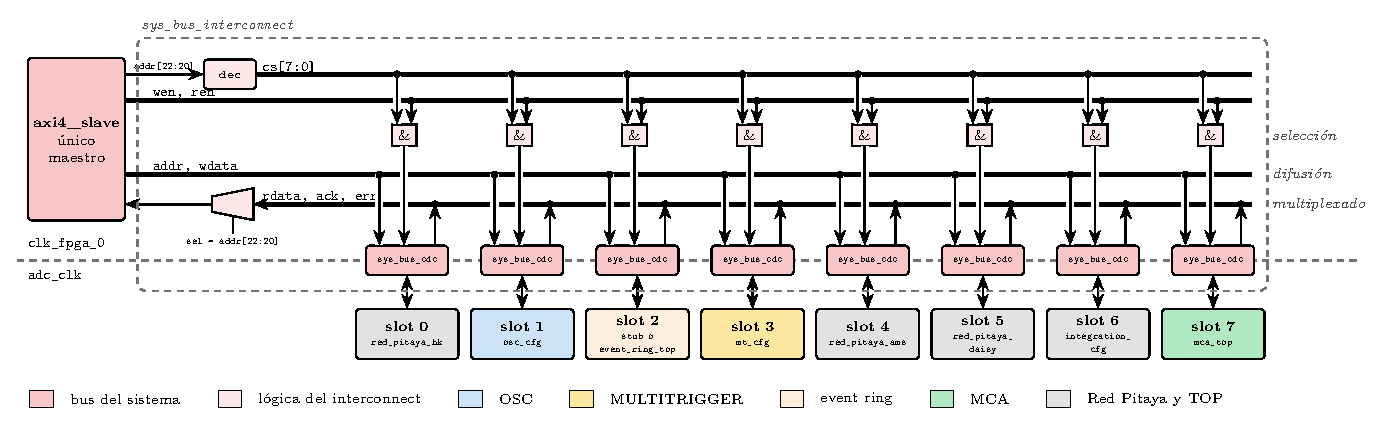
\includegraphics{cap12_estructura_sys_bus}
\caption[Interconnect principal del bus custom de Pitaya]{%
Esquema del interconnect principal del bus custom de Pitaya: una topología en
estrella en la que \codigo{axi4\_slave} es el único maestro y los ocho slots son
los esclavos.\label{f:top-interconnect}}
\end{figure}

\subsection{Cambios realizados en el TOP original}
\label{S:top-cambios}

\begin{sloppypar}
Nuestro TOP, \codigo{event\_ring\_red\_pitaya\_top}, parte del TOP del proyecto
(\codigo{red\_pitaya\_top}, el de Red Pitaya con el osciloscopio ya
reemplazado por \codigo{rp\_scope\_mt\_com}). Las diferencias son:
\end{sloppypar}
\begin{enumerate}
  \item \textbf{El MCA en el slot 7} (\codigo{0x4070\_0000}).
  \item \textbf{Sin ecualizador} (\codigo{EN\_FILT = 0}): su lazo IIR no cierra
    timing a \qty{125}{\mega\hertz}.
  \item \textbf{Sin generador arbitrario (ASG)} en el slot 2. Su lugar lo
    comparten dos módulos, que reparte \codigo{sys\_bus\_split}: el
    \codigo{event\_ring} (\codigo{0x4020\_0000}), que escribe sus ventanas a la
    DDR por HP2, y \codigo{gen\_pulsos} (\codigo{0x4021\_0000}), que maneja la
    entrada del DAC y la fuente de disparo ASG del multitrigger.
  \item \textbf{Sin captura del OSC a DDR} (\codigo{EN\_AXI = 0}): la reemplaza
    el \codigo{event\_ring}, y HP0 y HP1 quedan en cero. La captura por BRAM del
    OSC sigue.
  \item \textbf{Sin PID} en el slot 3, que no se usa en este flujo. En su lugar
    va el multitrigger, que en \codigo{red\_pitaya\_top} ocupa el slot 7.
  \item \textbf{\codigo{integration\_cfg} en el slot 6} y un selector de nodo por
    consumidor en el datapath (Sec.~\ref{S:top-registros}).
\end{enumerate}

Se conservan a propósito la lista de puertos y los nombres de instancia
\codigo{i\_ams} y \codigo{sys\_bus\_interconnect}, porque las restricciones del
XDC se enganchan por esos nombres.

\subsection{Redes de reloj y de reset}
\label{S:top-relojes}

El TOP arma dos familias de relojes (Tabla~\ref{t:top-relojes}). La primera nace
del ADC: el oscilador de la placa maneja al ADC y entra a la PL, a
\qty{125}{\mega\hertz}, por el par diferencial \codigo{adc\_clk\_i}. Con él se
alimenta una PLL~\cite{UG472} (\codigo{red\_pitaya\_pll}), de la que salen, por
buffers globales (BUFG), el reloj de la adquisición, los del DAC y el del enlace
serie. Todo el procesamiento propio (OSC, MT, MCA, \codigo{gen\_pulsos},
\codigo{event\_ring} e \codigo{integration\_cfg}) corre en \codigo{adc\_clk},
así que la muestra no cruza ningún dominio de reloj entre el ADC y el histograma
o el anillo. También corre en \codigo{adc\_clk} el \codigo{axi\_master} de HP2,
aunque esté dentro del módulo del PS. La segunda familia nace en el PS, que
genera sus relojes con sus propios PLL a partir de otro oscilador:
\codigo{fclk[0]}, de \qty{125}{\mega\hertz}, con el que corre el lado PS del
bus, y \codigo{fclk[3]}, de \qty{200}{\mega\hertz}, que usa el enlace serie para
los retardos de entrada (IDELAY). En la Fig.~\ref{f:top-panorama} cada bloque
lleva su reloj cuando no es \codigo{adc\_clk}, y los cruces que necesitan
sincronizador están marcados.

\begin{table}[H]
\centering
\caption[Relojes del TOP]{%
Relojes del TOP. Los de la PLL salen todos del reloj del ADC y guardan relación
de fase entre sí; los del PS, no. La PLL genera además un reloj de PWM que en
este TOP no usa ningún bloque: el PDM corre en \codigo{adc\_clk}. La recepción
del enlace serie usa el reloj que llega del otro extremo por el cable
SATA.\label{t:top-relojes}}
\small
\begin{tabularx}{\textwidth}{|>{\raggedright\arraybackslash}p{0.25\textwidth}%
  |>{\raggedright\arraybackslash}p{0.2\textwidth}|c%
  |>{\raggedright\arraybackslash}X|}
\hline \encabezado \textbf{Reloj} & \textbf{Frecuencia} & \textbf{Origen} &
  \textbf{Lo usa} \\ \hline
\codigo{adc\_clk} & \qty{125}{\mega\hertz} & PLL & adquisición,
  procesamiento, lado PL del bus y puerto HP2 \\ \hline
\codigo{dac\_clk\_1x} & \qty{125}{\mega\hertz} & PLL & DAC: datos de los dos
  canales intercalados, selección y reset \\ \hline
\codigo{dac\_clk\_2x}, \codigo{dac\_clk\_2p} & \qty{250}{\mega\hertz}; el
  segundo, a $-45^\circ$ & PLL & DAC: escritura y reloj de salida \\ \hline
\codigo{ser\_clk} & \qty{250}{\mega\hertz} & PLL & enlace serie
  (\codigo{red\_pitaya\_daisy}), transmisión \\ \hline
\codigo{fclk[0]} & \qty{125}{\mega\hertz} & PS & lado PS del bus
  (\codigo{axi4\_slave}) \\ \hline
\codigo{fclk[3]} & \qty{200}{\mega\hertz} & PS & retardos de entrada del enlace
  serie \\ \hline
\end{tabularx}
\end{table}

Aunque \codigo{fclk[0]} y \codigo{adc\_clk} tienen la misma frecuencia nominal,
no salen de la misma PLL: cada uno viene de su propio oscilador. Son relojes
\textbf{plesiócronos}~\cite{Dally1998}: tienen la misma frecuencia nominal, pero
cada oscilador tiene su tolerancia y su deriva, así que la fase entre los dos se
corre lentamente y, con el tiempo, pasa por todos los valores. No se les puede
suponer ninguna relación de fase fija, y el cruce necesita un sincronizador
general, el mismo que haría falta entre dos relojes sin ninguna relación. Si
salieran de la misma PLL serían sincrónicos y alcanzaría con el análisis de
timing, como pasa entre \codigo{adc\_clk} y los relojes del DAC.

El cruce lo hace el interconnect, con un \codigo{sys\_bus\_cdc} por slot que pasa
cada transacción de \codigo{fclk[0]} a \codigo{adc\_clk} y su respuesta de
vuelta, por un handshake con sincronizadores de varios
flip-flops~\cite{Cummings2008}. Por eso el bus admite una transacción a la vez
por slot y cada acceso se lleva unos pocos ciclos. Las restricciones del XDC no
suponen ninguna relación de fase entre los dos relojes: sólo acotan, a un
período, el retardo del camino hasta el primer flip-flop de cada sincronizador.
La respuesta de lectura cruza registrada: el esclavo deja el dato fijo en el
ciclo del ack y \codigo{sys\_bus\_cdc} lo congela antes de pasarlo al PS. Los
otros dos cruces los resuelve el propio PS en sus puertos~\cite{UG585}: GP0
corre en \codigo{fclk[0]} y HP2 en \codigo{adc\_clk}, y el PS pasa cada
transacción a sus relojes internos.

Cada dominio tiene su propio reset (\codigo{adc\_rstn}, \codigo{dac\_rst},
\codigo{dac\_axi\_rstn}, \codigo{pwm\_rstn}), registrado en su reloj. Todos salen
de \codigo{frstn[0]}, el reset de la PL que maneja el PS, y del enganche de la
PLL: el reset se mantiene activo mientras el PS mantenga \codigo{frstn[0]} y
durante una cuenta de ciclos después de que la PLL engancha, así ningún módulo
arranca con el reloj todavía inestable. Si la PLL pierde el enganche, el TOP la
resetea desde el dominio de \codigo{fclk[0]}, que no depende de ella. El estado
de \codigo{pll\_locked} y de \codigo{adc\_rstn} se puede leer desde
\codigo{integration\_cfg}.

\subsection{Datapath y cálculo de tiempo muerto en integración}
\label{S:top-datapath}

En la Fig.~\ref{f:top-datapath} se presentan los flujos principales de datos
dentro de la integración.

\begin{figure}[H]
\centering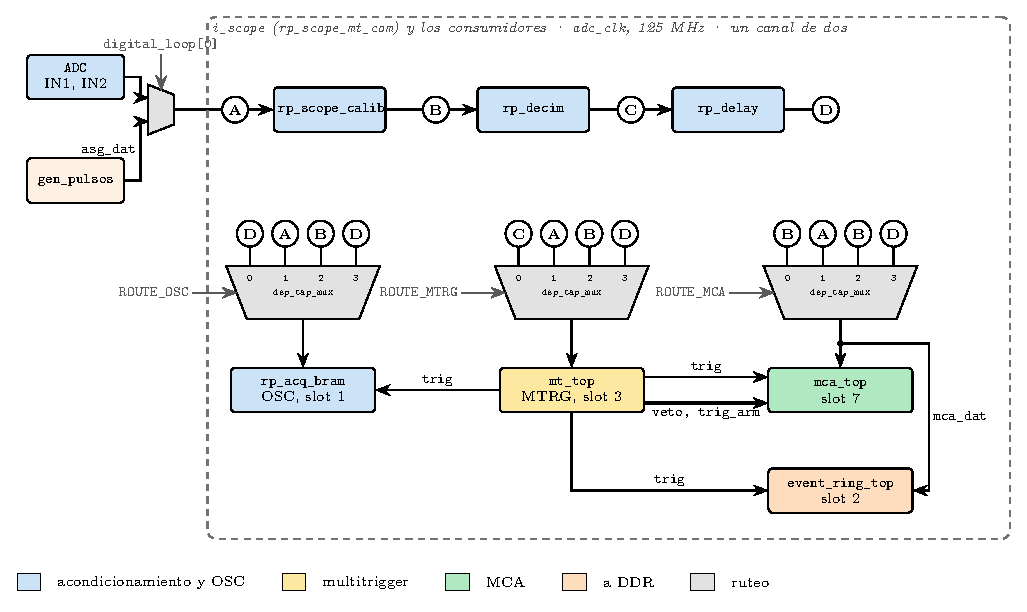
\includegraphics{cap12_datapath_top}
\caption[Datapath del módulo de integración]{%
Datapath del módulo de integración. Hay una sola cadena de acondicionado por
canal (calibración, diezmado, retardo) con cuatro nodos (A a D). El OSC, el
multitrigger y el MCA tienen cada uno su \codigo{dsp\_tap\_mux} 4:1, que elige
en runtime con su \codigo{ROUTE\_*}; cada entrada lleva su código de tap (0 a 3)
y la letra del nodo, y la 0 es el nodo nativo, el valor de reset. El
\codigo{event\_ring} no tiene selector: toma lo mismo que el MCA
(\codigo{mca\_dat}). A la izquierda, el lazo digital: con
\codigo{digital\_loop[0]} la cadena toma los pulsos de \codigo{gen\_pulsos} en
lugar del ADC. Abajo, lo que el multitrigger da a los otros consumidores: el
flanco \codigo{trig} a los tres, y \codigo{veto} y \codigo{trig\_arm}, niveles,
sólo al MCA.\label{f:top-datapath}}
\end{figure}

Hay una sola cadena de acondicionamiento por canal: calibración de ganancia y
offset (\codigo{rp\_scope\_calib}), diezmado (\codigo{rp\_decim}) y retardo de
disparo (\codigo{rp\_delay}). El ecualizador del proyecto de Red Pitaya
(\codigo{osc\_filter}) no está en nuestro TOP (\codigo{EN\_FILT = 0}), porque su
lazo IIR no cierra timing a \qty{125}{\mega\hertz}, y tampoco la captura del OSC
a DDR (\codigo{EN\_AXI = 0}), que reemplaza el \codigo{event\_ring}. Los
consumidores (OSC, MT, MCA y \codigo{event\_ring}) no tienen una cadena cada
uno: toman la muestra de uno de los cuatro nodos de esa misma cadena
(Tabla~\ref{t:top-nodos}). Para eso el OSC, el MT y el MCA tienen cada uno su
propio selector 4:1, \codigo{dsp\_tap\_mux}, que el software configura en tiempo
de ejecución con los registros \codigo{ROUTE\_*} de \codigo{integration\_cfg}.
Son tres selectores independientes, no una matriz de conmutación. El
\codigo{event\_ring} no tiene selector propio: toma la misma muestra que el MCA.
La entrada 0 de cada selector es el nodo \textbf{nativo}, el que el consumidor
tenía cableado antes de que existiera el selector, y es el valor de reset: sin
configurar nada, el datapath es idéntico al original.

\begin{table}[H]
\centering
\caption[Nodos de la cadena de acondicionamiento]{%
Nodos de la cadena de acondicionamiento; $R$ es el factor de diezmado. Cada nodo
es un prefijo de la misma cadena. El C sólo lo alcanza el MT, como nativo, y por
eso no tiene código de \codigo{tap\_sel}.\label{t:top-nodos}}
\small
\begin{tabularx}{\textwidth}{|c|l|>{\raggedright\arraybackslash}X|l|c%
  |>{\raggedright\arraybackslash}p{0.17\textwidth}|}
\hline \encabezado \textbf{Nodo} & \textbf{Señal} & \textbf{Etapas que acumuló}
  & \textbf{Ritmo} & \codigo{tap\_sel} & \textbf{Nativo de} \\ \hline
A & \codigo{adc\_calib\_in} & ninguna: la muestra cruda & 125~MSPS & 1 & ---
  \\ \hline
B & \codigo{adc\_dec\_in} & calibración & 125~MSPS & 2 & MCA y
  \codigo{event\_ring} \\ \hline
C & \codigo{adc\_dly\_in} & + diezmado & $125/R$~MSPS & --- & MT \\ \hline
D & \codigo{adc\_bram\_in} & + retardo & $125/R$~MSPS & 3 & OSC \\ \hline
\end{tabularx}
\end{table}

El selector arrastra el par (dato, valid): los nodos posteriores al diezmado
entregan una muestra cada $R$ ciclos con su estrobo, y los consumidores lo
respetan. Es combinacional a propósito: registrarlo correría el dato un ciclo
respecto de las señales de control de cada consumidor y, en modo nativo, el
hardware dejaría de ser idéntico al original.

Hay dos consecuencias para el uso. Como el \codigo{event\_ring} toma lo mismo
que el MCA, \codigo{ROUTE\_MCA} mueve a los dos. Y el MT toma por defecto el nodo
C, posterior al diezmado, así que diezmar para ver una ventana más larga en el
OSC también diezma la señal con la que se disparan el MCA y el ring, salvo que
se cambie \codigo{ROUTE\_MTRG}.

A la izquierda de la Fig.~\ref{f:top-datapath} está el lazo digital: con el bit
0 de \codigo{digital\_loop}, en \codigo{red\_pitaya\_hk}, la cadena toma los
pulsos de \codigo{gen\_pulsos} en lugar de las muestras del ADC, y todo el
datapath ve el estímulo del generador sin pasar por la etapa analógica.

\subsection{Registros de integración}
\label{S:top-registros}

El slot 6 lo ocupa \codigo{integration\_cfg}, un módulo propio que no existe en
el proyecto de Red Pitaya. Su función es que el software \textbf{descubra} el
sistema en lugar de suponerlo: qué bitstream está cargado, qué módulos trae y en
qué slot vive cada uno. Hace falta porque el mapa no es el mismo en todos los
bitstreams del proyecto. Sus registros se agrupan en cuatro bloques
(Tabla~\ref{t:top-registros}).

\begin{table}[H]
\centering
\caption[Bloques de registros de \codigo{integration\_cfg}]{%
Bloques de registros de \codigo{integration\_cfg} (base
\codigo{0x4060\_0000}).\label{t:top-registros}}
\small
\begin{tabularx}{\textwidth}{|>{\raggedright\arraybackslash}p{0.2\textwidth}%
  |>{\raggedright\arraybackslash}p{0.2\textwidth}%
  |>{\raggedright\arraybackslash}X|}
\hline \encabezado \textbf{Bloque} & \textbf{Offset} & \textbf{Contenido}
  \\ \hline
Identificación & \codigo{0x000}--\codigo{0x018} & \codigo{MAGIC}
  (\codigo{\textquotedbl INTG\textquotedbl}), versión y hash de git del commit
  del que salió el bitstream (160 bits) \\ \hline
Descripción del sistema & \codigo{0x020}--\codigo{0x02C} & \codigo{MODULES}
  (qué módulos hay), \codigo{SLOTS} (en qué slot está cada uno) y
  \codigo{CAPS\_*} (parámetros de síntesis: canales, anchos, tamaños de los
  histogramas) \\ \hline
Ruteo del datapath & \codigo{0x030}--\codigo{0x03C} & \codigo{ROUTE\_OSC},
  \codigo{ROUTE\_MTRG} y \codigo{ROUTE\_MCA}: nodo de cada consumidor
  (\codigo{[1:0]}) y habilitación (\codigo{[8]}). \codigo{ROUTE\_RING} existe
  pero no está conectado \\ \hline
Control global & \codigo{0x040}--\codigo{0x044} & \codigo{run},
  \codigo{clear} y \codigo{soft\_reset}, todavía sin consumidores; estado de
  \codigo{pll\_locked} y \codigo{adc\_rstn} \\ \hline
\end{tabularx}
\end{table}

Los registros de identificación y de descripción salen de parámetros de
síntesis, así que no cuestan flip-flops: son constantes cableadas al
multiplexor de lectura. El hash de git lo inyecta el script de construcción como
parámetro, de modo que el bitstream sabe de qué commit salió sin que nadie lo
anote. \codigo{libmca} lee estos registros para calcular la dirección de cada
módulo (Sec.~\ref{S:sw-libmca}).

% Bibliografía de este capítulo. Va al final del archivo, siempre.
\bibliografiacapitulo

%%% Local Variables:
%%% mode: latex
%%% TeX-master: "template"
%%% End:
